\documentclass[12pt]{article}
\linespread{1.5}
\pdfminorversion=6

\usepackage{booktabs}
\usepackage{tabularx}
\usepackage{caption}
\usepackage[flushleft]{threeparttable}
\usepackage{threeparttablex}

\usepackage[english]{babel}
\usepackage{float,color}
\usepackage[pdftex]{graphicx}
\usepackage{hyperref}
\usepackage{graphicx,scalerel}
\hypersetup{colorlinks,linkcolor=black,urlcolor=blue,citecolor=black}
\usepackage{amssymb}
\usepackage{amsmath}
\usepackage{placeins}
\usepackage[format=hang,font=normalsize,labelfont=bf]{caption}
\usepackage[margin=1in]{geometry}
\usepackage{url}
\usepackage{listings}
\usepackage{amsxtra}
\usepackage{setspace}
\usepackage{authblk}
\usepackage{csquotes}

% Bibliography stuff
\usepackage[
hyperref=true,
giveninits=true, % render first and middle names as initials
uniquename=init,
maxcitenames=3,
maxbibnames=99,
style=authoryear,
dashed=false, % re-print recurring author names in bibliography
natbib=true,
useprefix=true, % for inclusion of 'de' 'da' in surname
urldate=long,
backend=biber,
style=apa]{biblatex}
\addbibresource{bibliography.bib}

% adds space above row
\newcommand{\customlinespace}{\addlinespace[.1cm]}

% command for all table/figure notes
\newcommand{\Fignote}[1]{
	\begin{tablenotes}[para,flushleft]\footnotesize
		\textit{Note}: #1
	\end{tablenotes}
}

% stars
\newcommand{\sym}[1]{\rlap{#1}}

% note addendem for fixed effects
\newcommand{\FEnote}{All specifications include household and calendar-week-by-method-of-payment fixed effects. }

% note addendem for regression tables
\newcommand{\Regnote}{Standard errors in parentheses are clustered at household level. ***, **, and * indicate significance at the 1, 5, and 10 percent critical levels, respectively.}


% Title page stuff
\title{The Effect of the 2008 Economic Stimulus Payments on Nutrient Demand}
\author{Zachary A. Goodman\thanks{zgoodman@ucsd.edu.
I thank Jeffrey Clemens, Gordon Dahl, Melissa Famulari, Craig McIntosh, Katherine Meckel, and numerous seminar participants for their comments and suggestions.
My analyses are calculated based in part on data from Nielsen Consumer LLC and marketing databases provided through the NielsenIQ Datasets at the Kilts Center for Marketing Data Center at The University of Chicago Booth School of Business.
The conclusions drawn from the NielsenIQ data are those of my own and do not reflect the views of NielsenIQ.
NielsenIQ is not responsible for, had no role in, and was not involved in analyzing and preparing the results reported herein.}}
\affil{University of California, San Diego}
\date{This version: June 2021}

\begin{document}
\maketitle

\begin{abstract}
In this paper I examine the effects of receiving an economic stimulus payment (ESP) as part of the Economic Stimulus Act of 2008 on demand for nutrients. The ESPs, averaging about \$900, were distributed at quasi-random intervals over a 12-week time span depending on the last two digits of each taxpayer's Social Security number. I combine Nielsen Consumer Panel scanner data with UPC-level Nutrition Facts data and survey data that allows me to observe when NCP panelists received their ESPs and how much of each nutrient the household purchased over time. I find no evidence of changes in purchases by households with liquid savings. Liquidity constrained households, on the other hand, experience large increases in purchases of all nutrients, but particularly those considered unhealthful at current average levels by the USDA. The findings suggest that one-time transfers are unlikely to improve healthfulness of nutrient bundles purchased. More research is warranted to examine the effects of repeated transfers on nutrient demand.
\end{abstract}

\pagebreak

%%%%%%%%%%%%%%%%%%%%%%%%%%%%%%%
% Introduction
%%%%%%%%%%%%%%%%%%%%%%%%%%%%%%%
\doublespacing

\section{Introduction} \label{introduction}

The US spends about \$100 billion annually on programs designed to address food insecurity including the Supplemental Nutrition Assistance Program, Special Supplemental Nutrition Program for Women, Infants, and Children, and school meal programs.
These programs serve tens of millions of Americans: one in four uses a program offered by the US Department of Agriculture (USDA) Food and Nutrition Service at least once in a year \parencite{usdafns}.
Additionally, food insecurity and poor nutrition are often cited by politicians as justification for transfer programs.
Moreover, what we eat and drink plays a large role in health outcomes including obesity, which costs taxpayers north of \$200 billion dollars annually \parencite{cawley2012medical}.

Unconditional cash transfers (UCTs) have been proposed as ways to address poverty without spending resources on means testing \parencite{hanna2018universal} or increase aggregate consumption thereby helping reducing the duration of a recession \parencite{broda2014economic}.
However, little is known how UCTs affect nutritional choices in developed countries.
In this paper, I examine one such UCT, economic stimulus payments (ESPs) dispersed as part of the Economic Stimulus Act of 2008 (hereafter ESA), on demand for nutrients.
These ESPs were sent to households starting May 2008 in an effort to increase spending and reduce the duration of the recession caused by the 2007 financial crisis.
In total, over \$100 billion in ESPs were sent to 130 million taxpayers in 2008.
Fortuitously, the IRS decided when each taxpayer would receive her ESP using the last two digits of her Social Security number, which is effectively random assigned.\footnote{Social Security applicants are assigned the last four digits of their Social Security numbers sequentially within their the geographic area and group, which determine the first seven digits of their number.} The random timing of the ESP allows for identification of causal effects, which other authors such as \textcite{broda2014economic} have exploited to estimate the impact of receiving an ESP on consumption.
I use a similar approach to estimate the impact of receiving an ESP on demand for nutrients.

To estimate this effect, I calculate household-level nutrient purchases over time using data from the Nielsen Consumer Panel (NCP), which provides household-level purchase data at the barcode level for about 60,000 households over several years.
I merge these panel data with barcode-level Nutrition Facts data to observe quantities of each nutrient purchased per household over time.
Finally, I observe when panelists receive their ESPs using a special survey constructed by \textcite{broda2014economic} answered by NCP panelists before and during the period of time that ESPs were distributed.

I find that during the concurrent week the ESP is received, households increase total spending by 6\% and only increase spending on food by a modest, statistically insignificant amount.
However, households that do not have at least two months of income as liquid assets see large, significant effects on purchases of food.
These households increase their purchases of all nutrients, but the effects are heterogeneous.
Notably, carbohydrates and sugar increase more than other nutrients while protein and fiber increase the least.
These findings are consistent with the Permanent Income Hypothesis and the "wealthy hand-to-mouth" theory of \textcite{kaplan2014model}.
Additionally, these findings suggest that one-time, large income shocks are unlikely to improve nutritional quality, at least for populations similar to the sample studied, or perhaps developed countries more broadly.

The remainder of the paper is organized as follows.
Section \ref{background} provides a background of the policies enacted and related literature.
Sections \ref{methods} and \ref{data} introduce the methods and data used, respectively.
Section \ref{results} summarizes our results.
Section \ref{discussion} discusses those results and concludes.

%%%%%%%%%%%%%%%%%%%%%%%%%%%%%%%
% Background
%%%%%%%%%%%%%%%%%%%%%%%%%%%%%%%
\section{Background and Related Literature} \label{background}

In this section, I review the policy studied as well as the literature on the effects of ESPs in the United States and the demand for nutritious foods.

\subsection{Economic Stimulus Act of 2008} \label{2008esa}

First I provide background on the Economic Stimulus Act of 2008.
The ESA was signed into law by President George W.
Bush on February 13, 2008, which promised to provide ESPs to taxpayers who filed a 2007 tax return.
Each eligible taxpayer received between \$300 and \$600 if filing single or twice that amount if filing jointly, depending on tax liability in 2007 \parencite{house2008}.
To be eligible for an ESP, one must have earned at least \$3,000 in income in 2007 and have a sufficiently low income.
Adjusted gross income beyond a threshold of \$75,000 per qualifying adult phased out ESP benefits at a rate of 5\%.
Additionally, each dependent child increased one's ESP by \$300.
In total, the program disbursed about \$100 billion in payments to 130 million taxpayers \parencite{parker2013consumer}.

Although signed into law in February, taxpayers did not begin to receive ESPs until May.
For those taxpayers who provided direct deposit information, the IRS distributed electronic transfers of ESPs during a three-week period starting in late April.
For the remaining taxpayers, the IRS mailed paper checks during a nine-week period starting in early May through July.
In advance of sending the ESP, the IRS mailed recipients a notice that an ESP would be arriving soon.
The week a taxpayer received her ESP was determined by the last two digits of her Social Security number, which as mentioned earlier is assigned as good as randomly.
Hence, the \textit{timing} of receiving an ESP is random conditional on transfer method (electronic vs mail).
It is important to note that the amount of the ESP is \textit{not} random, nor is whether or not one receives an ESP.
Hence, identification of causal effects in this paper comes from comparing those who receive their ESP early to those who receive their ESP later, regardless of amount, conditional on transfer method.

\subsection{Unconditional cash transfers in the United States}

Here I review papers that examine causal effects of UCTs in the US \textcite{johnson2006household} use the quasi-random timing of tax rebate checks sent to households as part of the Economic Growth and Tax Relief Reconciliation Act of 2001 to estimate the effects of income shocks on consumption.
Using a unique set of questions added to the Consumer Expenditure Survey after passage of the 2001 Tax Act, they observe when households receive their payments.
Similar to the ESPs distributed in 2008, the timing of payments in 2001 depended on one's SSN, and hence the timing of receipt is as good as randomly assigned.
The authors find that households spent about two-thirds of their rebates over the six months following receipt on nondurable goods.

\textcite{broda2014economic} conduct the survey of Nielsen Consumer Panel households that I use in this paper to observe if and when households receive their stimulus payments, how much they received, and some information about preferences and how the household intends to spend their payments.
The authors find that households do not respond to news about the incoming payment but that aggregate spending rises by 10\% the week after the payment is received.
Additionally, spending remains higher for the three months following receipt of the payment, and the response is greatest for households that report low liquid wealth and low income.
In another paper, \textcite{parker2013consumer} add additional survey questions to the Consumer Expenditure Survey related to receipt of 2008 ESPs.
The authors find that households spent between 50 - 90\% of the payments, with about a third of that spent on nondurable goods.

\textcite{kaplan2014model} construct a model that can explain the smaller consumption response in 2008 vs 2001, which they detail in \textcite{kaplan2014tale}.
The authors describe ``wealthy hand-to-mouth" households who hold large amount of wealth mostly as illiquid assets.
These households display large marginal propensities to consume upon receiving a positive income shock but not upon receiving news of the shock, which runs counter to conventional hypotheses that uses a one-asset framework and ignore the liquidity of such an asset.
The key theoretical takeaway that I examine in this work is that liquidity constrained households, even those with significant savings, may experience consumption changes upon receiving an ESP.

\subsection{Demand for nutrients}

Here I review empirical work on demand for ``healthy" (non-sugar carbohydrates, fiber, unsaturated fats) and ``unhealthy" nutrients (saturated fats, sugar, sodium).\footnote{\textit{Healthy} in this context is guided by recommendations from US government agencies, such as the USDA's \textit{Dietary Guidelines for Americans} \citeyear{usda2021}, which are guided by current average levels of nutrient consumption in the US.}.
\textcite{allcott2019food} examine whether entrance of a supermarket to a ``food desert" reduces nutritional inequality between wealthy and poorer households.
The authors find that entrance of a new store does not significantly reduce nutritional inequality, which follows from the observation that households travel far to purchase groceries.
A closer proximity store simply changes where the households make their purchases and modestly helps households through decreased transit costs and increased variety.
The authors also find that moving to a healthier neighborhood does not make a large dent in nutritional inequality over several years following the move.
Finally, the authors report that providing poorer households with the same prices available to higher income households would reduce nutritional inequality by at most 10\% while the remaining 90\% is driven by differences in demand.
They suggest subsidizing healthy groceries, at a cost of 15\% of the budget for SNAP, to eliminate nutritional inequality.

Other authors have provided alternative explanations for preferences for nutritious foods.
\textcite{hut2020determinants} finds that migrants are mostly unaffected by local differences in demand for nutritious foods shortly after moving, but within three to four decades, about half of the difference in healthfulness is closed.
\textcite{harding2017effect} use structural modeling to estimate the impact of nutrient-specific taxes on demand, which they estimate using data from the NCP.
They find that a 20\% tax on fat, sugar, and salt reduces demand for that nutrient by 30.25\%, 16.41\%, and 10.03\%, respectively, all of which are more effective than are taxes on product classes (like sugar-sweetened beverages).
\textcite{griffith2017importance} report that decreased salt intake observed in the UK is due to firms reformulating products and not because of consumers choosing products with less salt.
In a recent paper, \textcite{harris2020online} finds that the introduction of an online shopping service modestly reduces the share of budget spent on sweets and candies but no evidence of improvement across other measures of healthfulness.

%%%%%%%%%%%%%%%%%%%%%%%%%%%%%%%
% Data
%%%%%%%%%%%%%%%%%%%%%%%%%%%%%%%
\section{Data} \label{data}

I identify the causal effects of UCTs on nutrient demand using several data sources.
I start with data from the Nielsen Homescan Survey, a nationally-representative panel that allows me to observe household-level food purchases and demographic data for about 60,000 households in 2008.
Households in the panel are provided a barcode scanner by Nielsen, who asks households to scan all items purchased.
To incentivize households to scan items, Nielsen offers a rewards catalog, which provides panelists higher value rewards the longer they remain in the sample.\footnote{The median household stays in the sample for about seven years.}

When scanning barcodes, Nielsen panelists are asked to provide information about the store where the product was purchased and the price of the item.
Prices are automatically recorded for products purchased at a Nielsen partner retail outlet as the average price during the week the panelist purchased the product.
Panelists are asked to manually input the price of products made at non-partner retail outlets.
For barcodeless products like some produce and bakery items, Nielsen provides a reference booklet with barcodes associated with a photo and description of a product.\footnote{``Reference card goods'' are underreported in the Nielsen data, and Nielsen provides sampling weights for researchers who choose to include reference card goods in their analysis that upweight households that scan reference card items.} In practice, households may choose to omit reporting certain purchases or forget to scan and do not report all purchases \parencite{einav2010recording}.
Hence I report coefficient estimates as percent changes.
Provided the degree of underreporting in the homescan data is not correlated with ESP timing, the treatment effect estimates should not be biased by this measurement error of all purchases.

To observe nutrition information, I match the UPC codes associated with each Nielsen product with barcode-level nutrition data.
I then collapse these data to observe total quantities of each nutrient purchased per household per week.
The nutrition information come from three sources.
The first source is from Syndigo, who license their nutrition dataset covering over 220,000 products containing information from the Nutrition Facts panel, ingredients list, and general product attributes like brand, size, and description.\footnote{Over 2,000 consumer applications have licensed these data, as have other researchers such as \textcite{dubois2014prices} who also match these data to Nielsen products.} The second source is the US Department of Agriculture's FoodData Central, which provides product-specific nutrient information.
The final source is from images of products provided by major online retailers, from which I hand-record nutrition information from pictures of the Nutrition Facts panel.

I follow an imputation process similar to that of \textcite{dubois2014prices} to label each purchased product with nutrient information.
I begin by dropping non-food products, alcohol, tobacco, weight-loss/diet aids, and reference card goods.\footnote{Reference card goods do not have barcodes and are generally underreported by panelists.
Additionally, they are reported as \textit{counts} as opposed to weights, thereby making it difficult to label these products with correct nutrition information.} % As a robustness check we examine whether RC purchases change as a function of the tax.
I then match Nielsen products to Syndigo nutrients, covering about 62.7\% of purchased products.
I next match products without a direct match to those that share the same product description, brand, product module,\footnote{Nielsen defines over 1,000 product categories called \textit{product modules}.}, size type,\footnote{``Size type'' is whether the product is measured in counts versus volume versus weight, which is generally (but not always) consistent within product module.} flavor, variety, type, formula, and style, which adds 22.2\% to the matched data.
After that, I allow matches across brands, including storebrand goods, which do not have matches in the Syndigo data.
This step matches 8.5\% of purchased products.
The next step relaxes the flavor, variety, type, formula, and style restrictions, labeling 4.3\% of products.
I then impute with product module for ones that have sufficient labeled observations, which covers 2.1\% of products.
Finally, I manually label the remaining 0.3\% of products using the USDA and online retailer data sources.
After aggregating to the household-week level, I topcode each nutrient measure at the 99th percentile for all values greater than the 99th percentile to reduce the influence of outliers.
 %TODO citation of another paper that does this

Finally, I use the survey constructed by \textcite{broda2014economic} to observe when panelists received their ESPs.
The survey was sent to all NCP households who met Nielsen's reporting requirement, who were offered rewards points to answer.
The instructions asked that the survey be answered by ``the adult most knowledgeable about your household's income tax returns".
The first wave of the survey asked households for details about whether they had received a payment or if not, when they expected to receive a payment, if any.
Subsequent waves followed up with households that had not yet received a payment but expected to in the future or were not sure if they would receive a payment.
For households who reported receiving a payment, the survey asked for the amount and date the ESP was received as well as how the respondents' household anticipated spending or saving the money.
The survey also asked all respondents a series of questions related to liquidity and savings.
For a detailed description of the survey questions and timing, see the Appendix of \textcite{broda2014economic}.

Of the approximately 60,000 households receiving the survey, 80\% responded, providing a pre-trimmed sample of about 48,000.
By necessity, I drop all households who report not receiving an ESP or omit a date of receipt, which removes about 20\% of respondents.
Additionally, I follow \textcite{broda2014economic} in dropping households who report obviously wrong or inconsistent information.
Specifically, I drop households who report receiving an ESP before ESPs of their type were distributed, those who report receiving an ESP at a date prior to an earlier survey wave in which they reported not receiving an ESP, and those who report receiving an ESP in a future date after the survey's timestamp.
I also drop households who receive their ESPs later than the IRS-published disbursement schedules, which is possible but not random which households received their ESPs late.
Finally, I drop households who do not make purchases both before and after receipt of their ESP, which is necessary to include household fixed effects.
Very few households did not report purchases both before and after receipt, so this step likely has minimal impact on results.
The resulting sample includes 19,961 households of which 9,190 received their ESP by direct deposit, 10,744 by mail, and the remaining 27 unsure.\footnote{For those households unsure of method of receipt, I used the union of eligibility dates across both methods of receipt when trimming the sample.}

Clearly the sample remaining is not randomly selected.
However, if the timing of receipt for this sample is random conditional on receipt type, estimated effects are unbiased, and the effects are representative of trimmed sample.
There may be a few concerns that could lead to nonrandom timing of receipt.
First, it is possible that households do not report their receipt dates correctly.
Second, even if households report the dates correctly, we cannot observe when households were supposed to receive their payments.
As such, it is possible that there is nonrandom selection where those reporting receiving their payments late, albeit still inside the permissible period, were supposed to receive their payments sooner.
To give some confidence that households are reporting correctly, I plot the daily counts of reported receipt dates in Figure \ref{ts_esp}.
Interestingly, the spikes early in the distribution period line up with the distribution dates reported by the IRS for direct deposit.
Hence, I proceed under the assumption that all households reported correct receipt dates, with the caveat that the reported dates are perhaps more accurate in the direct-deposit subsample.
Furthermore, the inclusion window for mailed checks is much larger, which provides greater opportunity for nonrandom selection of late recipients into the sample.

I present descriptive statistics of the selected sample in Tables \ref{table_summary_cat} and \ref{table_summary_num}, which may be helpful for deciding whether the results may generalize to other populations and grasping the magnitude of effects.

%%%%%%%%%%%%%%%%%%%%%%%%%%%%%%%
% Methods
%%%%%%%%%%%%%%%%%%%%%%%%%%%%%%%

\section{Methods} \label{methods}

In this section, I describe the empirical strategies used in this paper.

\subsection{Effect on payment on nutrient demand}

I use a stacked event study design to estimate the impact of receiving an ESP on purchases.
The primary specification is as follows:

\begin{align}
	y_{it} = \text{ESP}_{i(t)} + \alpha_i + \gamma_t + \epsilon_{it} \label{spec_es}
\end{align}

where $y_{it}$ is the total purchases of a food or nutrient $y$ by household $i$ during week $t$, $\alpha_i$ is a household fixed effect, $\gamma_t$ are week fixed effects, and $\epsilon_{it}$ is an unobserved error term.
$\text{ESP}_{i(t)}$ is a set of indicators for week since the household received its ESP, and I omit the week two weeks prior to when the household receives its check such that all coefficients are relative to that week.\footnote{I omit two weeks instead of the week immediately prior to allow for anticipatory effects.} I additionally drop a second relative-week indicator far in advance of treatment, which is required to avoid multicollinearity as discussed in \textcite{borusyak2017revisiting}.\footnote{Doing so implicitly assumes the coefficient is zero, which is reasonable if there are no pretreatment trends.
Another option is to not include household fixed effects.} Identification of the indicator dummies comes from timing of the ESPs, which is assigned as-good-as random conditional on ESP type (paper check or direct deposit) and receiving the payment when expected, as described in detail in Section \ref{2008esa}.
As such, I interact $\gamma_t$ by method of payment indicators as well as estimate my primary specifications restricting the sample to only those who receive their ESP by the same method.
Under unconfoundedness and SUTVA, the coefficients $\text{ESP}_{i(t)}$ for $i(t) \geq 0$ identify the (weighted) average treatment effect on the treated (ATT) of receiving an ESP on purchases of $y$ after $t$ weeks.
I use the inverse hyperbolic sine of levels of $y$ such that the coefficients can be interpreted as percent changes.
When reporting average effects over multiple weeks, I average the relevant indicator coefficients.

In this setting, the \textit{timing} of treatment is randomly assigned, and treated units remain ``treated" for all following periods.
\textcite{athey2021design} show that causal effects in such a ``staggered adoption design" can be estimated using the standard differences-in-differences (DID) estimator and interpreted as a weighted average of the average effect of changing the adoption date.
The authors also prove that the clustered bootstrap provides a conservative estimate of the variance of the coefficients of interest.
\textcite{sun2020estimating} examine the event-study specification, which I use in this paper, and demonstrate that, even in settings where all units are treated, treatment effect estimates remain unbiased provided that the pattern of treatment effect does not change over time.
I follow the guidance of that work as well as the principles shared in other recent papers \parencite{goodman2018difference, callaway2020difference, de2020two} when performing robustness checks.
Of note, I do not include relative-time dummies beyond the last period for which I have at least one untreated group (set of households who have not yet received their impending ESPs).
This limits my post-treatment observation period to 12 weeks with the full sample, 9 weeks with the paper-check sample, and 4 weeks with the direct deposit sample.

\subsection{Heterogeneity}

According to the Permanent Income Hypothesis, those with sufficient liquidity should not change their nutrient purchases dramatically upon receiving an ESP.
To examine heterogeneous treatment effects of the ESP, I adjust \ref{spec_es} to include an interaction term:

\begin{align}
	y_{it} = \text{ESP}_{i(t)} + \beta_t \text{I}_{i} * \text{ESP}_{i(t)} + \alpha_i + \gamma_t + \epsilon_{it} \label{spec_het}
\end{align}

where $\text{I}_{i}$ is an indicator equal to 1 when a household has a time-invariant characteristic of interest, such as having at least two months of income saved in liquid assets.
Note that time-invariant, in this setting, requires that the characteristic be constant during the periods studied, which is assumed to be true for all (annually-updated) Nielsen-provided demographic information.
$\beta_t$, the parameter of interest in this specification, is the average difference in the outcome variable during week $t$ for household who have the time-invariant characteristic of interest.

%%%%%%%%%%%%%%%%%%%%%%%
% Results
%%%%%%%%%%%%%%%%%%%%%%%

\section{Results} \label{results}

In this section I present results using the methodology discussed in Section \ref{methods} estimated using data described in Section \ref{data}.

\subsection{Effect on panelist behaviors}

I first estimate the effects of receiving an ESP on panelist behaviors, such as number of trips taken, items scanned, and total amount spent using Equation \ref{spec_es}.
I present my findings in Table \ref{table_behaviors_all} and select event study coefficient plots in Figure \ref{es_behaviors_all}.
In general, I find small, often insignificant effects in the first few weeks after receipt, and zero effect beyond that.
Specifically, like \textcite{broda2014economic}, I find significant effects on total spending in the first week after receipt; however, I find more modest effects of about 6\%.
I find insignificant and close to zero effects on total amount spent on scanned items, scanned food, and quantities of both.
Finally, I find a tight zero effect on number of trips, suggesting that on average, the ESP did not increase the number of trips taken by panelists.

I second estimate Equation \ref{spec_het} using liquidity constraints as the interaction variable of interest.
Specifically, I can observe whether a household reports having at least two months of income accessible in liquid assets.
I report results in Table \ref{table_behaviors_inter} and event study relative-time coefficients in the left panel of Figure \ref{es_interaction}.
Interestingly, all outcomes of interest are statistically significantly significant and large.
Compared to high liquidity households, low liquidity households increased their total expenditures by 17\% on all purchases, 15\% on scanned goods, and 12\% on food items.
These households purchased about 10\% more items and went on 5\% more trips in the first week.
By the second week, the effects fade somewhat but remain significant for total expenditures and trips.
The results are driven by direct deposit panelists, though the results are directionally positive for check-recipients as well.

\subsection{Effect on nutrient demand}

Next I examine the effects of receiving an ESP on nutrients purchased.
The procedure is similar to that discussed in the previous section with panelist behaviors: I start by estimating the average effect across the sample and then estimate the difference in treatment effects for the low-liquidity subsample.

The story is similar for nutrients.
When estimating treatment effects across the entire sample, as can be seen in Table \ref{table_nutrients_all} and Figure \ref{es_nutrients_all}, the average effects are small and insignificant.
However, when including an interaction term for low liquidity households, the average effects are nearly all significant and large during the week of receipt, as can be seen in Table \ref{table_nutrients_inter}.
Notably, calories increase by 19\%, which can be explained by increases in fat, carbohydrates, and protein of 11\%, 16\%, and 13\%, respectively.
Alcohol (volume) purchases increase by about 10\%, which may carry externalities that could be nontrivial in the aggregate.
By the second week, the average effects have tapered off and are often insignificant, though still directionally positive and often large.

%%%%%%%%%%%%%%%%%%%%%%%
% Discussion
%%%%%%%%%%%%%%%%%%%%%%%
\section{Discussion and Conclusion} \label{discussion}

While conditional cash transfers in the U.S. are well studied, there is limited research on the effects of unconditional cash transfers.
Given that ESPs can be sent quickly to help reverse contractionary economic periods, political leaders are increasingly talking about Universal Basic Income, and ESPs have recently been deployed during the COVID-19 epidemic, it is important to understand how ESPs affect consumer decisions that have downstream health consequences.
Little is known about how ESPs affect nutritional choices, which is troubling given the large public investment in programs that assist nutritional choices and costs incurred by nutrition-related health complications.

In this paper I exploit the ESPs sent as part of the Economic Stimulus Act of 2008, which was designed to increase consumer spending and help reduce the downturn from the 2007 financial crisis.
This policy delivered payments to US taxpayers at quasi-random delivery times, allowing for identification of causal effects using the exogenous timing.
In the sample studied, these payments averaged \$900 and arrived between late April and late July 2008, allowing me to identify the effect of receiving an ESP up to 12 weeks early.
In general, I find evidence that the average effects on nutrient purchases were modest, which is consistent with the Permanent Income Hypothesis.
However, households with low amounts of liquid assets had large and significant increases of purchases of all nutrients, but particularly those the USDA has encouraged reducing consumption.
Collectively, I interpret this as evidence that one-time, large income shocks are unlikely to improve diet healthfulness in the short run and may even reduce healthfulness.
However, one may view this optimistically as evidence that households splurge on special occasions (e.g. receiving a large payment from the government) and may otherwise follow a comparatively healthier diet.

\subsection{Limitations}

This paper is primarily limited by data concerns, particularly reliance on self-reporting of ESP receipt date.
Besides containing measurement error, those who receive their payments later in the cycle (by factors other than random chance) may have unobservable factors that confound the treatment effect estimates.
I present some evidence that these populations are likely small, at least among those reporting direct deposit payments; alas, this error is not observable.
Second, the results are specific to the time period studied, namely the beginning of the worst economic recession in recent history.
It is possible that the results may look very different if, for example, payments were made during an expansionary period.
Third, the estimates are specific to a one-time transfer.
Further research is warranted for estimating the impact of repeat transfers on household nutrition, which would help policymakers predict nutrition-related health impacts of transfer programs like universal basic income.


\clearpage
\printbibliography

%%% TABLES

\singlespacing

% \clearpage
\begin{table} \begin{center}
                    \caption{Summary statistics, categorical variables}
                    \label{table_summary_cat}
\footnotesize
\newcolumntype{Y}{>{\raggedleft\arraybackslash}X}
\begin{tabularx} {14cm} {@{} l Y Y Y Y Y Y Y Y Y Y Y Y Y Y Y Y@{}} \\
\toprule
 & \multicolumn{3}{c}{At least two months income in liquid assets} \\
\cmidrule(l{.75em}){2-4} 
&Illiquid&Liquid&Total \\
\cmidrule(l{.75em}){2-2} \cmidrule(l{.75em}){3-3}\cmidrule(l{.75em}){4-4}
&\%&\%&\% \\
\midrule
Hours employment/week of male head of HH&&& \\
No head of this gender&28.05&26.76&27.22 \\
$<$ 30&2.45&2.92&2.76 \\
30 - 34&1.89&1.58&1.69 \\
$\geq$ 35&49.37&37.96&42.04 \\
Not employed&18.23&30.77&26.29 \\
\midrule
Hours employment/week of male head of HH&&& \\
No head of this gender&10.57&13.66&12.55 \\
$<$ 30&11.76&9.72&10.45 \\
30 - 34&4.64&3.82&4.11 \\
$\geq$ 35&38.87&30.42&33.45 \\
Not employed&34.16&42.37&39.44 \\
\midrule
Racial identity&&& \\
White&79.54&84.01&82.41 \\
Black&12.18&7.64&9.26 \\
Asian&1.64&3.59&2.89 \\
Other&6.64&4.76&5.44 \\
\midrule
Household income&&& \\
$<$\$35K&44.70&33.26&37.35 \\
\$35K - \$59,999&28.87&29.27&29.13 \\
\$60K - \$99,999&23.32&31.03&28.27 \\
$>$\$100K&3.11&6.44&5.25 \\
\midrule
Age of the (female) head of household&&& \\
$<$35&17.71&8.59&11.85 \\
35 - 49&39.88&22.92&28.99 \\
50-64&32.40&37.17&35.46 \\
65+&10.01&31.31&23.70 \\
\midrule
Education of the (female) head of household&&& \\
$<$ HS&4.50&3.27&3.71 \\
HS Grad&34.64&33.01&33.59 \\
Some College&33.28&29.22&30.67 \\
Bachelor's+&27.58&34.51&32.03 \\
\midrule
Any children $<$ 18&&& \\
No&60.78&80.36&73.36 \\
Yes&39.22&19.64&26.64 \\
\midrule
WIC indicator&&& \\
No&74.24&92.25&85.81 \\
Current&3.34&0.80&1.70 \\
Previously&22.42&6.96&12.48 \\
\midrule
Households &7,136&12,825&19,961 \\
\bottomrule
\addlinespace[.75ex]
\end{tabularx}
\par
\scriptsize{}
\normalsize
\end{center}
\end{table}

\clearpage
\begin{spacing}{1.0} \begin{table} \centering \caption{Summary statistics, numeric variables} \label{table_summary_num} \resizebox{\linewidth}{!}{%
\begin{threeparttable} \begin{tabular}{m{0.30\linewidth}*{6}{>{\centering\arraybackslash}m{0.09\linewidth}}} \toprule
                    &    Illiquid&            &      Liquid&            &       Total&            \\
                    &        mean&          sd&        mean&          sd&        mean&          sd\\
\midrule
ESP by check        &        0.45&        0.50&        0.54&        0.50&        0.50&        0.50\\
ESP by dir. dep.    &        0.54&        0.50&        0.46&        0.50&        0.49&        0.50\\
ESP amount          &      906.76&      555.96&      864.12&      516.83&      881.88&      533.89\\
Trips               &        3.12&        1.98&        2.95&        1.72&        3.02&        1.83\\
Total spent         &      129.75&       74.14&      117.66&       69.95&      122.70&       71.97\\
Total spent, scanned items&       93.35&       56.86&       83.24&       51.83&       87.45&       54.21\\
Total spent, scanned food&       46.44&       25.88&       41.77&       23.67&       43.72&       24.72\\
Scanned items       &       33.08&       17.98&       28.50&       16.06&       30.40&       17.03\\
Storebrand items    &        5.67&        4.87&        4.65&        3.98&        5.08&        4.40\\
Food items          &       23.64&       13.13&       20.50&       11.62&       21.80&       12.37\\
Items with deals    &        6.82&        9.39&        8.06&        9.71&        7.55&        9.60\\
Items with coupons  &        1.53&        2.79&        1.62&        2.75&        1.58&        2.77\\
Coupon value        &        2.50&        4.92&        2.67&        5.02&        2.60&        4.98\\
Calories            &     3920.57&     2400.06&     3146.84&     2021.15&     3469.10&     2219.98\\
Calories from fat   &      996.14&      582.96&      816.46&      506.29&      891.30&      546.77\\
Carbohydrates       &      652.20&      448.04&      510.45&      365.33&      569.49&      407.88\\
Cholesterol         &        0.14&        0.09&        0.12&        0.09&        0.13&        0.09\\
Fat                 &      110.05&       64.58&       90.15&       56.01&       98.44&       60.53\\
Fiber               &       31.34&       17.80&       28.47&       16.54&       29.66&       17.13\\
Protein             &       98.46&       55.49&       86.62&       50.39&       91.55&       52.90\\
Saturated fat       &       42.66&       25.61&       34.93&       22.26&       38.15&       24.02\\
Sodium              &        6.14&        3.55&        5.09&        3.10&        5.53&        3.33\\
Sugar               &      423.01&      354.94&      321.46&      276.92&      363.76&      315.79\\
Transfat            &        1.44&        1.18&        1.04&        0.94&        1.21&        1.07\\
\midrule
Households & 7,136 & & 12,825 & & 19,961 & \\
\bottomrule \end{tabular} \Fignote{Variables are at the household-week level. Nutrient variables are all in grams, except for calories. Finanical variables are all in nominal dollars. Statistics are weighted using each household's projection factor as provided by Nielsen.} \end{threeparttable}} \end{table} \end{spacing}


\clearpage
\begin{spacing}{1.0} 
\begin{table} \centering \caption{Effects of ESP receipt on behaviors} 
\label{table_behaviors_all} 
\resizebox{\linewidth}{!}{%
\begin{threeparttable} 
\begin{tabular}{m{0.30\linewidth} *{6}{>{\centering\arraybackslash}m{0.10\linewidth}}}
\toprule
& \multicolumn{3}{c}{First week} & \multicolumn{3}{c}{Two weeks}\\
 \cmidrule(l{.75em}){2-4} \cmidrule(l{.75em}){5-7}
                   Outcome &     All & Dir. Dep. &   Check &     All & Dir. Dep. &   Check \\
\midrule
               Total spent &  0.058\sym{*} &     0.074 &   0.044 &  0.067\sym{*} &     0.041 &   0.066 \\
                           & (0.034) &   (0.066) & (0.042) & (0.036) &   (0.082) & (0.044) \\
Total spent, scanned items &   0.024 &     0.018 &   0.024 &   0.036 &    -0.005 &   0.042 \\
                           & (0.032) &   (0.063) & (0.039) & (0.034) &   (0.077) & (0.041) \\
 Total spent, scanned food &   0.007 &     0.022 &   0.010 &   0.015 &     0.006 &   0.014 \\
                           & (0.030) &   (0.058) & (0.038) & (0.032) &   (0.071) & (0.040) \\
                     Trips &   0.010 &    -0.003 &   0.009 &   0.012 &    -0.016 &   0.016 \\
                           & (0.012) &   (0.023) & (0.015) & (0.012) &   (0.029) & (0.015) \\
             Scanned items &   0.016 &     0.024 &   0.014 &   0.021 &    -0.002 &   0.023 \\
                           & (0.026) &   (0.050) & (0.033) & (0.028) &   (0.061) & (0.034) \\
        Scanned food items &   0.010 &     0.014 &   0.016 &   0.012 &    -0.010 &   0.017 \\
                           & (0.026) &   (0.049) & (0.033) & (0.027) &   (0.060) & (0.034) \\
                
\midrule 
Households &  19,961 &     9,190 &  10,744 &  19,961 &     9,190 &  10,744 \\
\bottomrule
\end{tabular}
\Fignote{\FEnote \Regnote} 
\end{threeparttable}}
\end{table} 
\end{spacing}

\clearpage
\begin{spacing}{1.0} 
\begin{table} \centering \caption{Effects of ESP receipt on nutrients} 
\label{table_nutrients_all} 
\resizebox{\linewidth}{!}{%
\begin{threeparttable} 
\begin{tabular}{m{0.30\linewidth} *{6}{>{\centering\arraybackslash}m{0.10\linewidth}}}
\toprule
& \multicolumn{3}{c}{First week} & \multicolumn{3}{c}{Two weeks}\\
 \cmidrule(l{.75em}){2-4} \cmidrule(l{.75em}){5-7}
      Outcome &     All & Dir. Dep. &   Check &     All & Dir. Dep. &   Check \\
\midrule
     Calories &   0.005 &     0.047 &   0.009 &   0.025 &     0.009 &   0.027 \\
              & (0.056) &   (0.108) & (0.070) & (0.060) &   (0.135) & (0.074) \\
         Fats &   0.001 &     0.033 &  -0.002 &   0.006 &    -0.009 &   0.002 \\
              & (0.036) &   (0.068) & (0.045) & (0.038) &   (0.084) & (0.047) \\
Saturated fat &   0.019 &     0.050 &   0.015 &   0.020 &     0.014 &   0.014 \\
              & (0.030) &   (0.057) & (0.038) & (0.032) &   (0.071) & (0.040) \\
    Trans fat &  -0.001 &    -0.018 &   0.009 &  -0.005 &    -0.019 &  -0.000 \\
              & (0.014) &   (0.027) & (0.018) & (0.015) &   (0.031) & (0.018) \\
Carbohydrates &   0.008 &     0.042 &   0.012 &   0.021 &     0.010 &   0.020 \\
              & (0.045) &   (0.087) & (0.056) & (0.048) &   (0.108) & (0.060) \\
        Sugar &   0.034 &     0.070 &   0.039 &   0.035 &     0.042 &   0.037 \\
              & (0.043) &   (0.083) & (0.053) & (0.045) &   (0.102) & (0.056) \\
        Fiber &   0.004 &     0.017 &  -0.004 &   0.009 &    -0.017 &   0.001 \\
              & (0.029) &   (0.055) & (0.036) & (0.031) &   (0.068) & (0.038) \\
       Sodium &   0.007 &     0.003 &   0.010 &   0.006 &    -0.020 &   0.010 \\
              & (0.020) &   (0.037) & (0.025) & (0.021) &   (0.045) & (0.026) \\
      Protein &   0.007 &     0.019 &   0.008 &   0.018 &    -0.014 &   0.020 \\
              & (0.036) &   (0.068) & (0.044) & (0.038) &   (0.083) & (0.047) \\
      Alcohol &   0.025 &    0.086\sym{*} &   0.002 &   0.018 &     0.057 &   0.020 \\
              & (0.025) &   (0.048) & (0.032) & (0.026) &   (0.056) & (0.033) \\
  Cholesterol &   0.003 &     0.005 &   0.001 &   0.002 &     0.002 &   0.002 \\
              & (0.003) &   (0.005) & (0.003) & (0.003) &   (0.006) & (0.003) \\
   
\midrule 
Households &  19,961 &     9,190 &  10,744 &  19,961 &     9,190 &  10,744 \\
\bottomrule
\end{tabular}
\Fignote{\FEnote \Regnote} 
\end{threeparttable}}
\end{table} 
\end{spacing}

\clearpage
\begin{spacing}{1.0} 
\begin{table} \centering \caption{Effects of ESP receipt on behaviors, low liquidity households} 
\label{table_behaviors_inter} 
\resizebox{\linewidth}{!}{%
\begin{threeparttable} 
\begin{tabular}{m{0.30\linewidth} *{6}{>{\centering\arraybackslash}m{0.10\linewidth}}}
\toprule
& \multicolumn{3}{c}{First week} & \multicolumn{3}{c}{Two weeks}\\
 \cmidrule(l{.75em}){2-4} \cmidrule(l{.75em}){5-7}
                   Outcome &      All & Dir. Dep. &   Check &      All & Dir. Dep. &   Check \\
\midrule
               Total spent & 0.167\sym{***} &  0.254\sym{***} &   0.096 & 0.114\sym{***} &    0.194\sym{*} &   0.132 \\
                           &  (0.057) &   (0.088) & (0.082) &  (0.057) &   (0.115) & (0.082) \\
Total spent, scanned items & 0.151\sym{***} &  0.237\sym{***} &   0.089 &  0.106\sym{**} &    0.200\sym{*} &   0.115 \\
                           &  (0.054) &   (0.084) & (0.077) &  (0.054) &   (0.108) & (0.077) \\
 Total spent, scanned food & 0.124\sym{***} &  0.193\sym{***} &   0.095 &    0.079 &     0.167 &   0.092 \\
                           &  (0.052) &   (0.081) & (0.073) &  (0.052) &   (0.105) & (0.074) \\
                     Trips & 0.051\sym{***} &  0.067\sym{***} &   0.039 &   0.035\sym{*} &    0.072\sym{*} &   0.047 \\
                           &  (0.020) &   (0.031) & (0.029) &  (0.020) &   (0.041) & (0.029) \\
             Scanned items & 0.103\sym{***} &  0.160\sym{***} &   0.076 &    0.068 &     0.139 &   0.083 \\
                           &  (0.044) &   (0.069) & (0.064) &  (0.045) &   (0.088) & (0.064) \\
        Scanned food items & 0.092\sym{***} &  0.158\sym{***} &   0.068 &    0.055 &    0.152\sym{*} &   0.065 \\
                           &  (0.045) &   (0.070) & (0.063) &  (0.045) &   (0.089) & (0.064) \\
                
\midrule 
Households &   19,961 &     9,190 &  10,744 &   19,961 &     9,190 &  10,744 \\
\bottomrule
\end{tabular}
\Fignote{The first set of columns is $\beta_1$ from Equation \ref{spec_het} while 
the second set includes the average of $\beta_1$ and $\beta_2$. \FEnote \Regnote} 
\end{threeparttable}}
\end{table} 
\end{spacing}

\clearpage
\begin{spacing}{1.0} 
\begin{table} \centering \caption{Effects of ESP receipt on nutrients, low liquidity households} 
\label{table_nutrients_inter} 
\resizebox{\linewidth}{!}{%
\begin{threeparttable} 
\begin{tabular}{m{0.30\linewidth} *{6}{>{\centering\arraybackslash}m{0.10\linewidth}}}
\toprule
& \multicolumn{3}{c}{First week} & \multicolumn{3}{c}{Two weeks}\\
 \cmidrule(l{.75em}){2-4} \cmidrule(l{.75em}){5-7}
      Outcome &      All & Dir. Dep. &   Check &     All & Dir. Dep. &   Check \\
\midrule
     Calories &   0.186\sym{*} &  0.333\sym{***} &   0.125 &   0.123 &     0.296 &   0.137 \\
              &  (0.097) &   (0.152) & (0.136) & (0.097) &   (0.197) & (0.137) \\
         Fats &   0.109\sym{*} &  0.206\sym{***} &   0.042 &   0.071 &    0.219\sym{*} &   0.054 \\
              &  (0.062) &   (0.096) & (0.088) & (0.062) &   (0.124) & (0.089) \\
Saturated fat &  0.103\sym{**} &  0.197\sym{***} &   0.043 &   0.066 &    0.203\sym{*} &   0.053 \\
              &  (0.052) &   (0.081) & (0.074) & (0.053) &   (0.104) & (0.076) \\
    Trans fat & 0.051\sym{***} &    0.071\sym{*} &  0.063\sym{*} &   0.009 &     0.031 &   0.024 \\
              &  (0.025) &   (0.038) & (0.037) & (0.025) &   (0.048) & (0.037) \\
Carbohydrates & 0.163\sym{***} &  0.277\sym{***} &   0.136 &   0.112 &     0.249 &   0.142 \\
              &  (0.078) &   (0.123) & (0.110) & (0.079) &   (0.159) & (0.112) \\
        Sugar & 0.160\sym{***} &  0.254\sym{***} &   0.152 &   0.116 &    0.252\sym{*} &   0.156 \\
              &  (0.074) &   (0.116) & (0.104) & (0.075) &   (0.150) & (0.105) \\
        Fiber & 0.137\sym{***} &  0.196\sym{***} &   0.109 &  0.092\sym{*} &   0.202\sym{**} &   0.106 \\
              &  (0.051) &   (0.079) & (0.072) & (0.051) &   (0.101) & (0.073) \\
       Sodium & 0.109\sym{***} &  0.156\sym{***} & 0.098\sym{**} &  0.060\sym{*} &    0.130\sym{*} &   0.068 \\
              &  (0.035) &   (0.054) & (0.049) & (0.035) &   (0.068) & (0.050) \\
      Protein & 0.126\sym{***} &  0.215\sym{***} &   0.081 &   0.073 &     0.199 &   0.071 \\
              &  (0.061) &   (0.095) & (0.087) & (0.062) &   (0.121) & (0.088) \\
      Alcohol & 0.096\sym{***} &  0.159\sym{***} &   0.087 &  0.080\sym{*} &     0.093 &   0.080 \\
              &  (0.043) &   (0.068) & (0.058) & (0.044) &   (0.081) & (0.061) \\
  Cholesterol &    0.007 &     0.010 &   0.007 &   0.001 &     0.006 &   0.004 \\
              &  (0.005) &   (0.007) & (0.007) & (0.005) &   (0.009) & (0.007) \\
   
\midrule 
Households &   19,961 &     9,190 &  10,744 &  19,961 &     9,190 &  10,744 \\
\bottomrule
\end{tabular}
\Fignote{The first set of columns is $\beta_1$ from Equation \ref{spec_het} while 
the second set includes the average of $\beta_1$ and $\beta_2$. \FEnote \Regnote} 
\end{threeparttable}}
\end{table} 
\end{spacing}

%%% FIGURES

% esp receipt date
\clearpage
\begin{figure}[t]
\begin{center}
\caption{Dates ESP reported received}
\label{ts_esp}
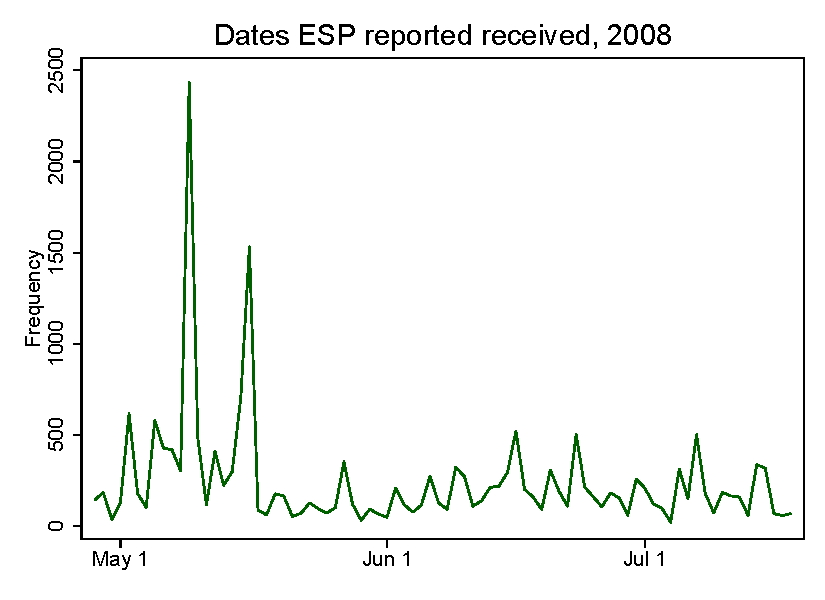
\includegraphics[width=1\textwidth, angle=0]{../figures/ts_esp.pdf}
\footnotesize
\end{center}
\end{figure}

% behaviors
\clearpage
\begin{figure}[t]
\begin{center}
\caption{Effects of ESP receipt on shopping behaviors}
\label{es_behaviors_all}
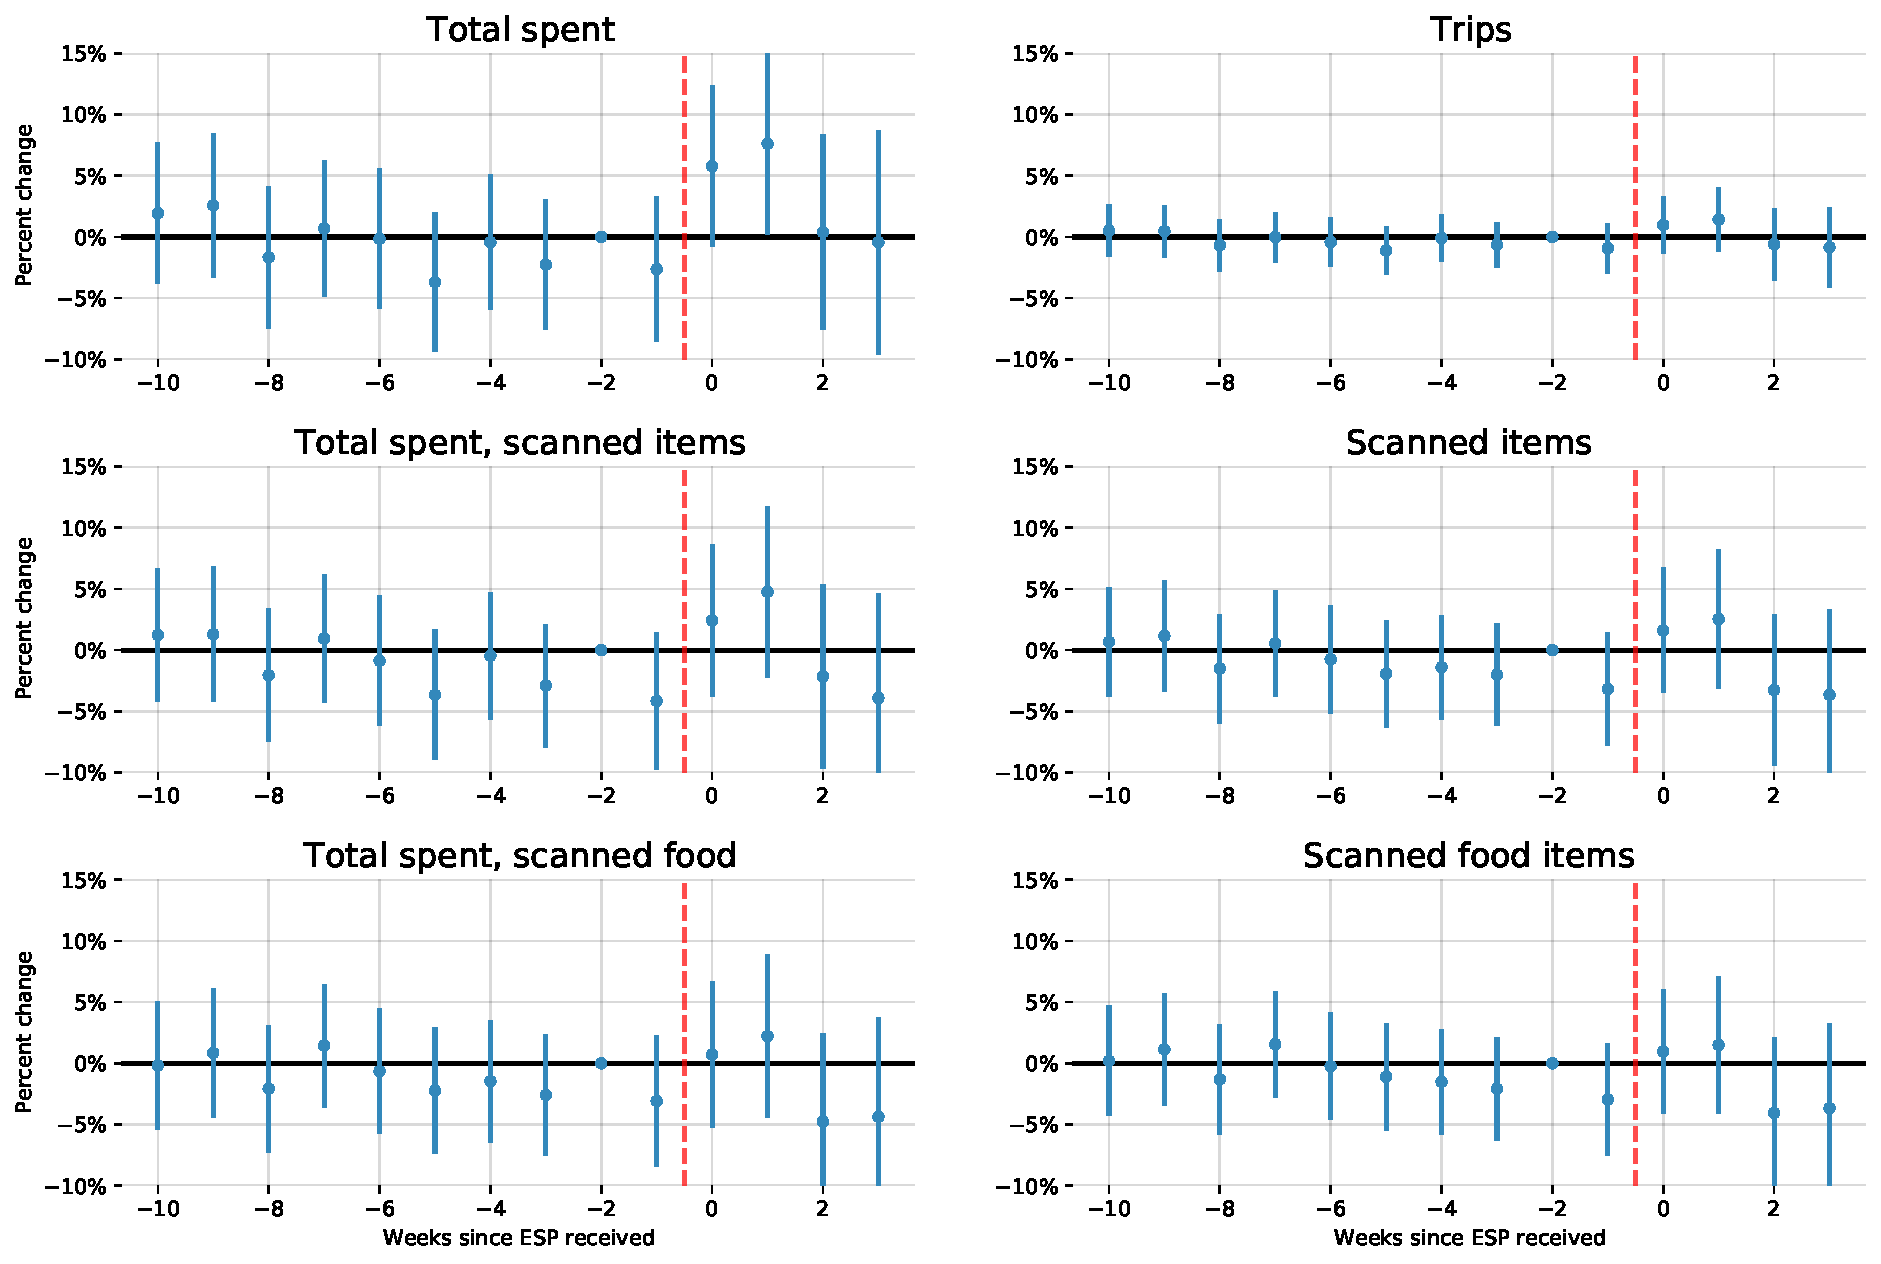
\includegraphics[width=1\textwidth, angle=0]{../figures/es_behaviors_all.pdf}
\footnotesize Each panel displays the weekly percent differences for the given outcome variable fit using Equation \ref{spec_es}. The regressions used include household and week-by-method-of-receipt fixed effects. Errors are clustered at the household level. \end{center}
\end{figure}

% nutrients
\clearpage
\begin{figure}[t]
\begin{center}
\caption{Effects of ESP receipt on nutrient purchases}
\label{es_nutrients_all}
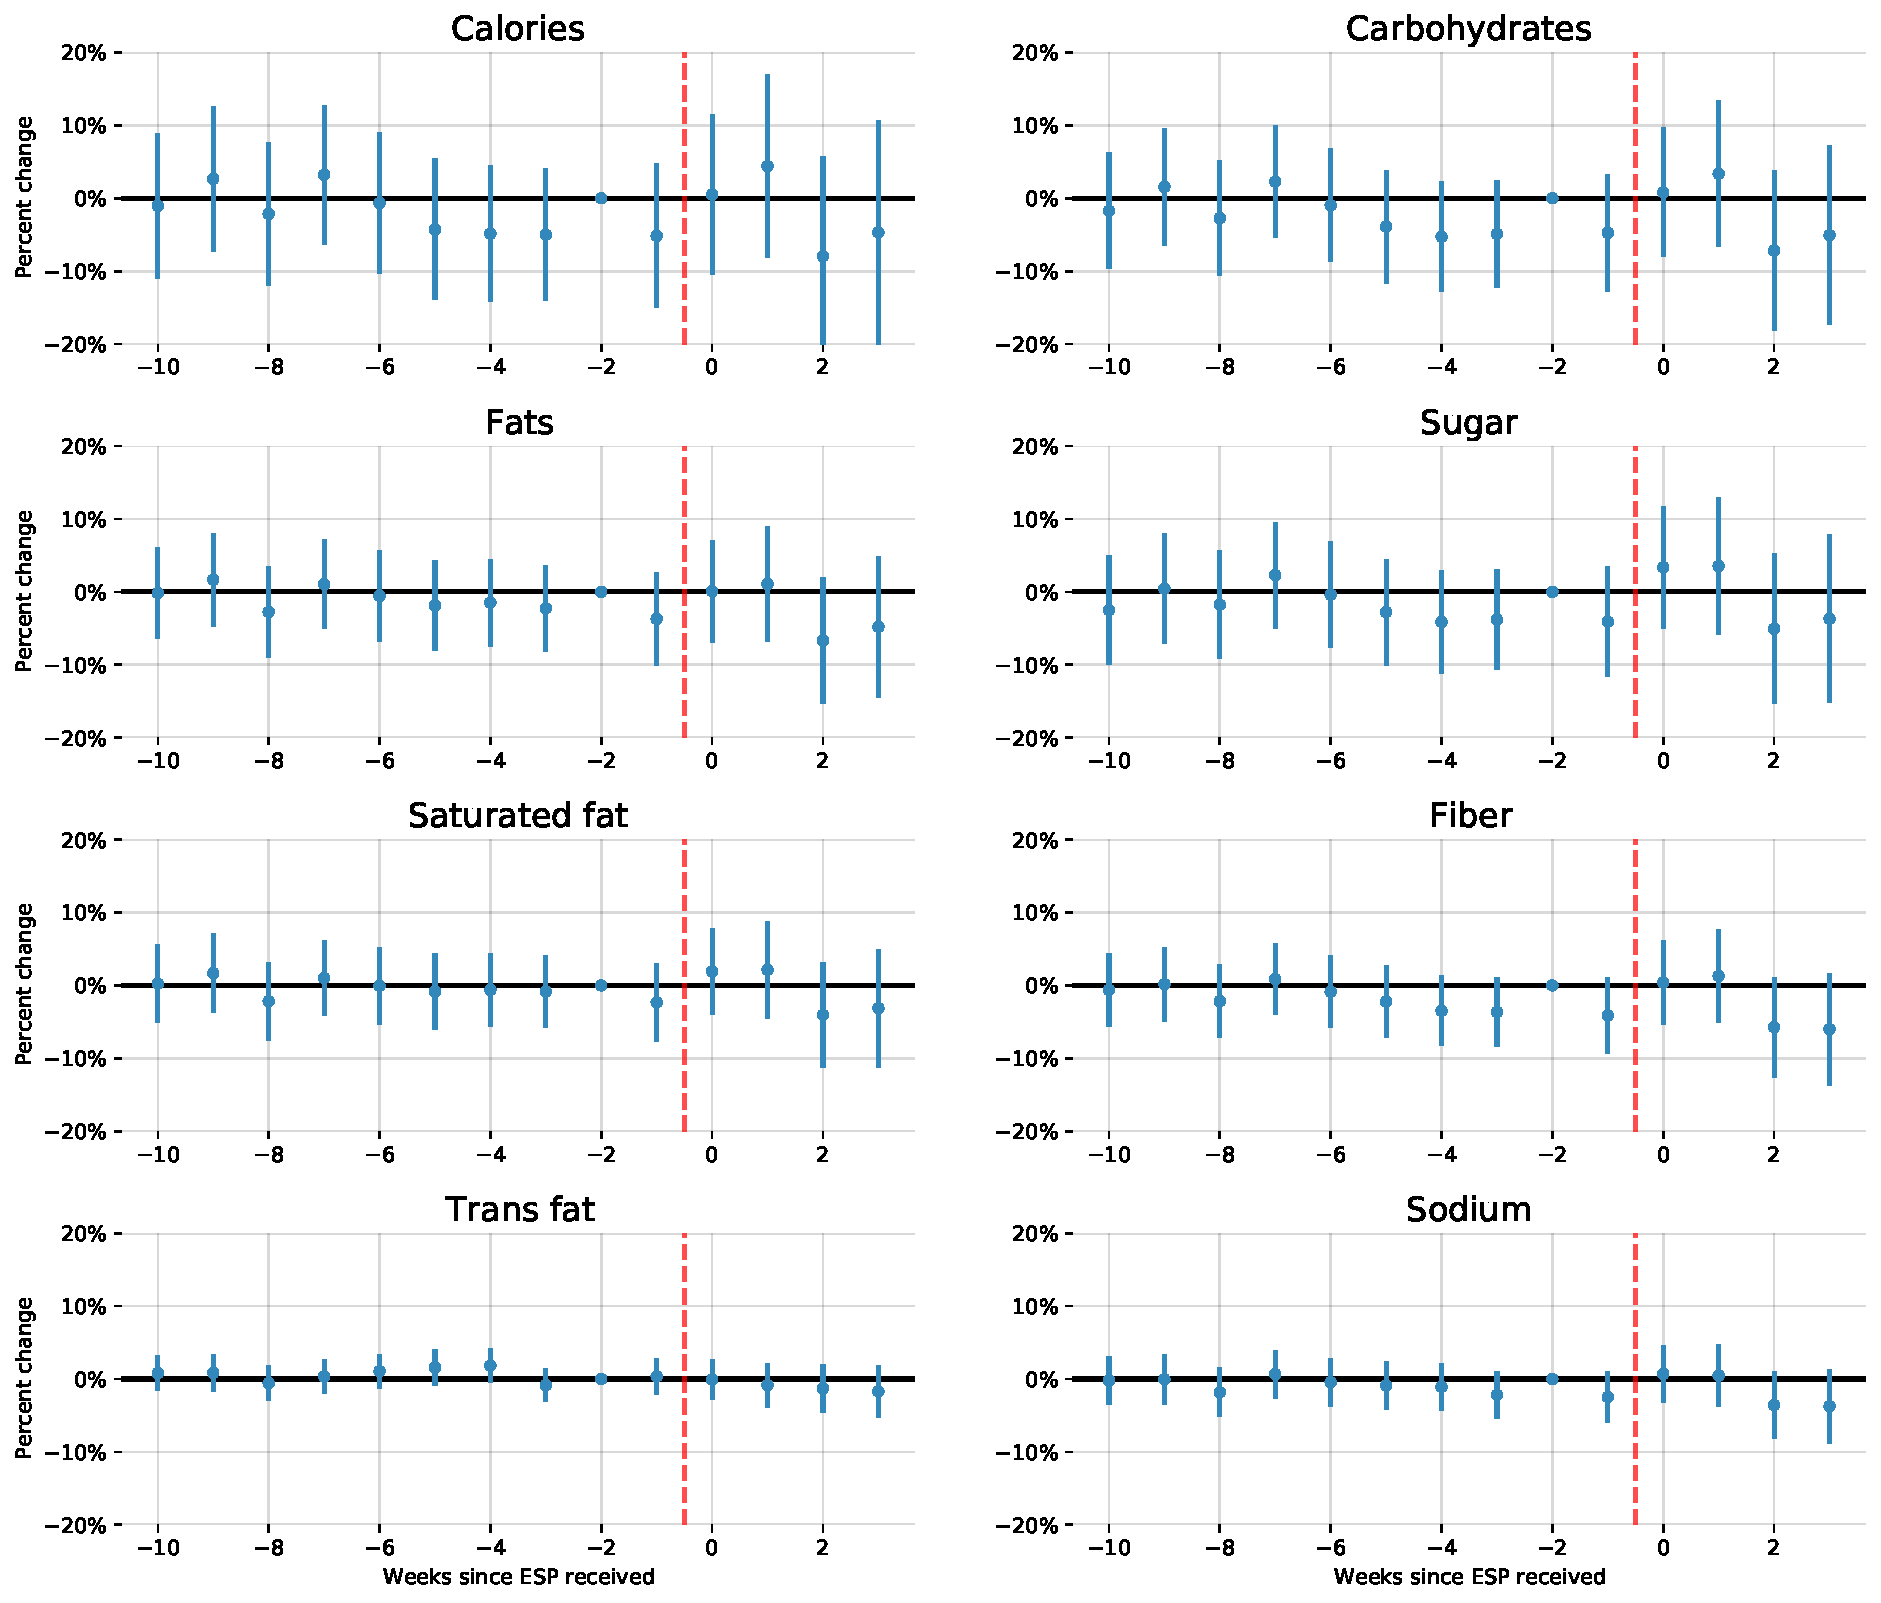
\includegraphics[width=1\textwidth, angle=0]{../figures/es_nutrients_all.pdf}
\footnotesize Each panel displays the weekly percent differences for the given outcome variable fit using Equation \ref{spec_es}. The regressions used include household and week-by-method-of-receipt fixed effects. Errors are clustered at the household level. \end{center}
\end{figure}

% interaction
\clearpage
\begin{figure}[t]
\begin{center}
\caption{Difference in effects of ESP receipt for low liquidity households}
\label{es_interaction}
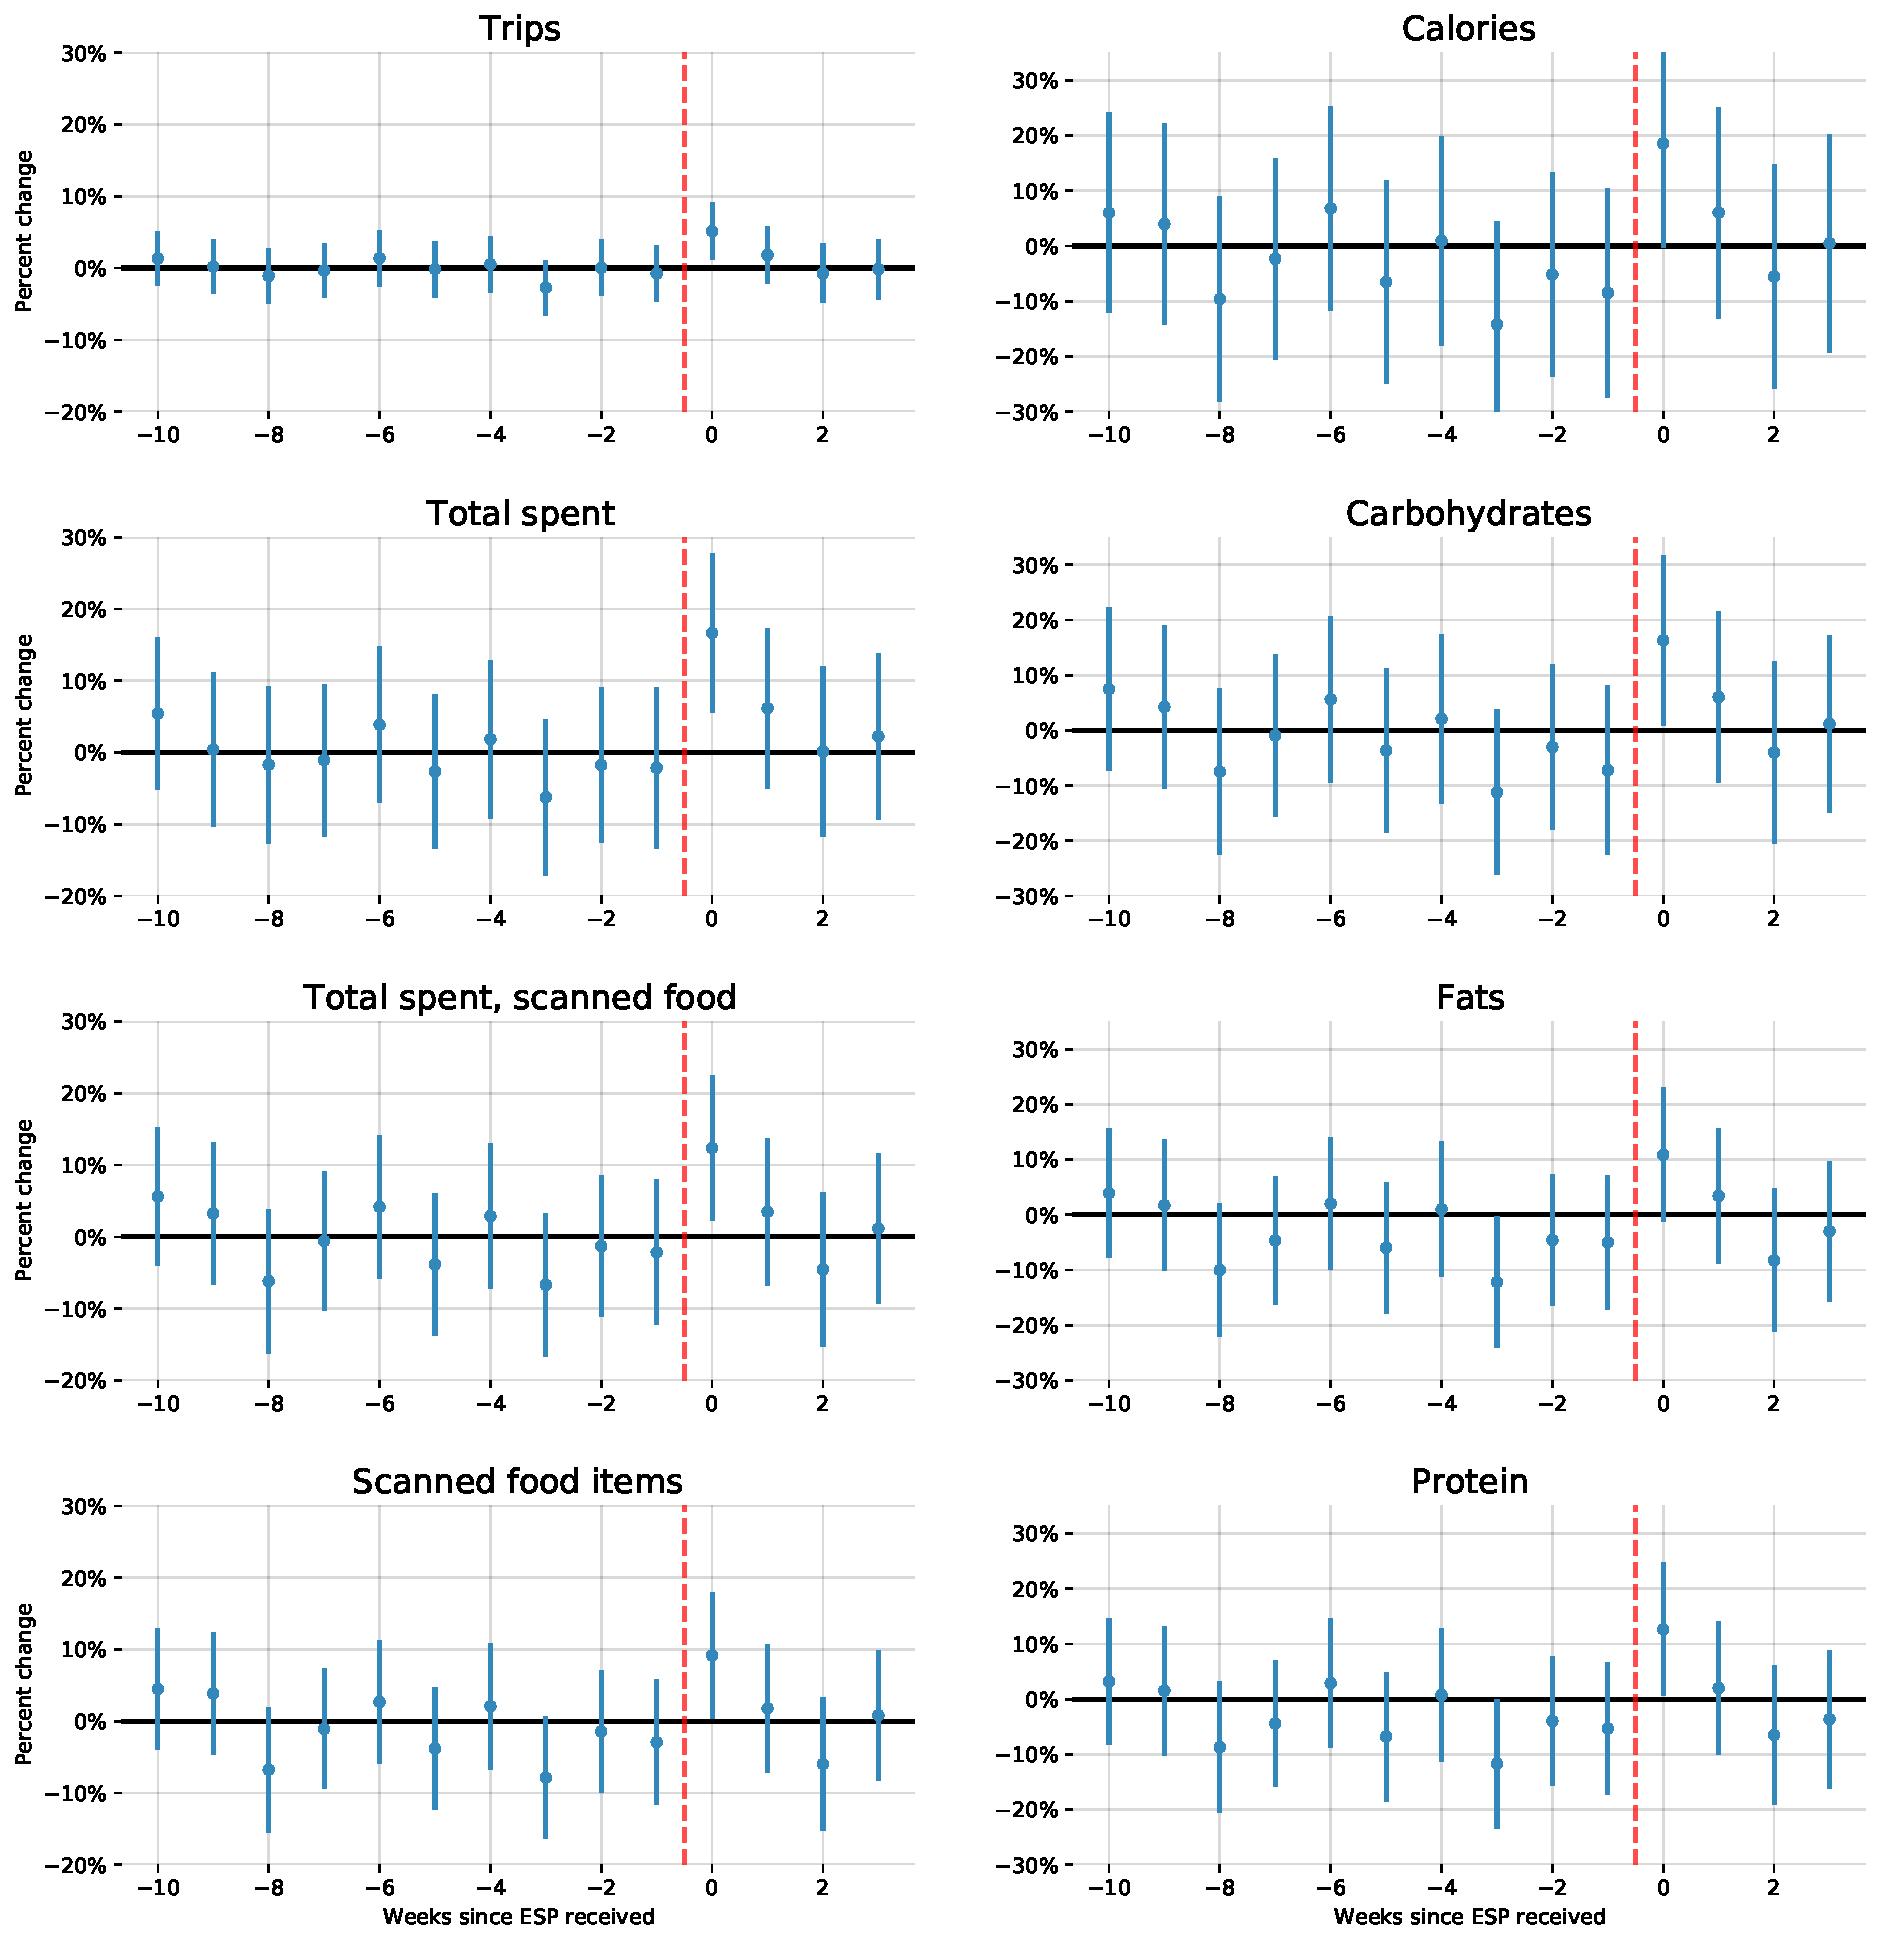
\includegraphics[width=1\textwidth, angle=0]{../figures/es_interaction.pdf}
\footnotesize Each panel displays $\beta_t$ from Equation \ref{spec_het}. The regressions used include household and week-by-method-of-receipt fixed effects. Errors are clustered at the household level. \end{center}
\end{figure}


% *****************************************************************
% Appendix
% *****************************************************************
\clearpage
\section*{Appendix}

\renewcommand{\thesubsection}{\Alph{subsection}}
\setcounter{table}{0}
\renewcommand{\thetable}{A\arabic{table}}
\setcounter{figure}{0}
\renewcommand{\thefigure}{A\arabic{figure}}

%%% TABLES

% \begin{spacing}{1.0}
\begin{table} \centering \caption{Effects of ESP receipt on behaviors, week of receipt}
\label{table_week_behaviors}
\begin{threeparttable}
\begin{tabular}{m{0.35\linewidth} *{3}{>{\centering\arraybackslash}m{0.15\linewidth}}}
\toprule
                   Outcome &      All & Dir. Dep. &   Check \\
\midrule
               Total spent & 0.167\sym{***} &  0.254\sym{***} &   0.096 \\
                           &  (0.057) &   (0.088) & (0.082) \\
Total spent, scanned items & 0.152\sym{***} &  0.237\sym{***} &   0.089 \\
                           &  (0.054) &   (0.084) & (0.077) \\
 Total spent, scanned food & 0.125\sym{***} &  0.193\sym{***} &   0.095 \\
                           &  (0.052) &   (0.081) & (0.073) \\
                     Trips & 0.052\sym{***} &  0.067\sym{***} &   0.039 \\
                           &  (0.020) &   (0.031) & (0.029) \\
             Scanned items & 0.103\sym{***} &  0.160\sym{***} &   0.076 \\
                           &  (0.044) &   (0.069) & (0.064) \\
        Scanned food items & 0.092\sym{***} &  0.158\sym{***} &   0.068 \\
                           &  (0.045) &   (0.070) & (0.063) \\

\midrule
Households &   19,961 &     9,190 &  10,744 \\
\bottomrule
\end{tabular}
\Fignote{\FEnote \Regnote}
\end{threeparttable}
\end{table}
\end{spacing}


% \clearpage
% \input{../tables/sodatilesozcook.tex}


%%% FIGURES

% Raw behavior data, weekly
\clearpage
\begin{figure}[t]
\begin{center}
\caption{Nutrient purchases over time by liquidity constraints}
\label{graph_raw_behaviors}
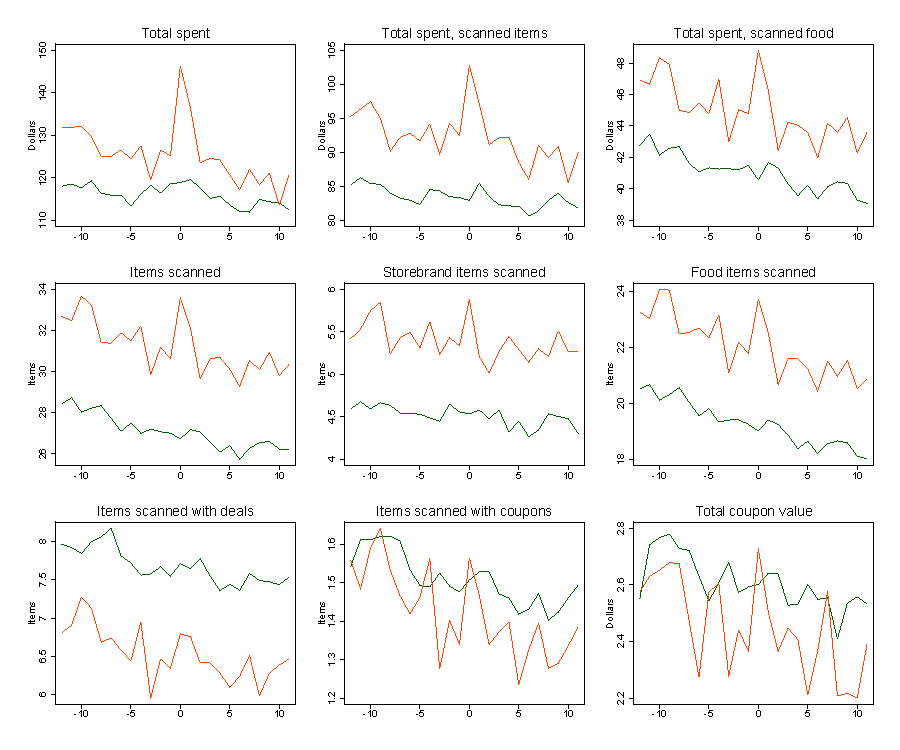
\includegraphics[width=1\textwidth, angle=0]{../figures/raw_behaviors_week.pdf}
\footnotesize Each panel displays weekly sums of different panelist behaviors averaged across panelists in the sample by whether they have at least two months of income in liquid assets.
Orange (generally top) line is liquidity-constrained households, green (generally bottom) line is those with liquidity.
Averages are weighted by panelist projection factors provided by Nielsen.
\end{center}
\end{figure}

% Raw nutrient data, weekly
\clearpage
\begin{figure}[t]
\begin{center}
\caption{Nutrient purchases over time by liquidity constraints}
\label{graph_raw_nutrients}
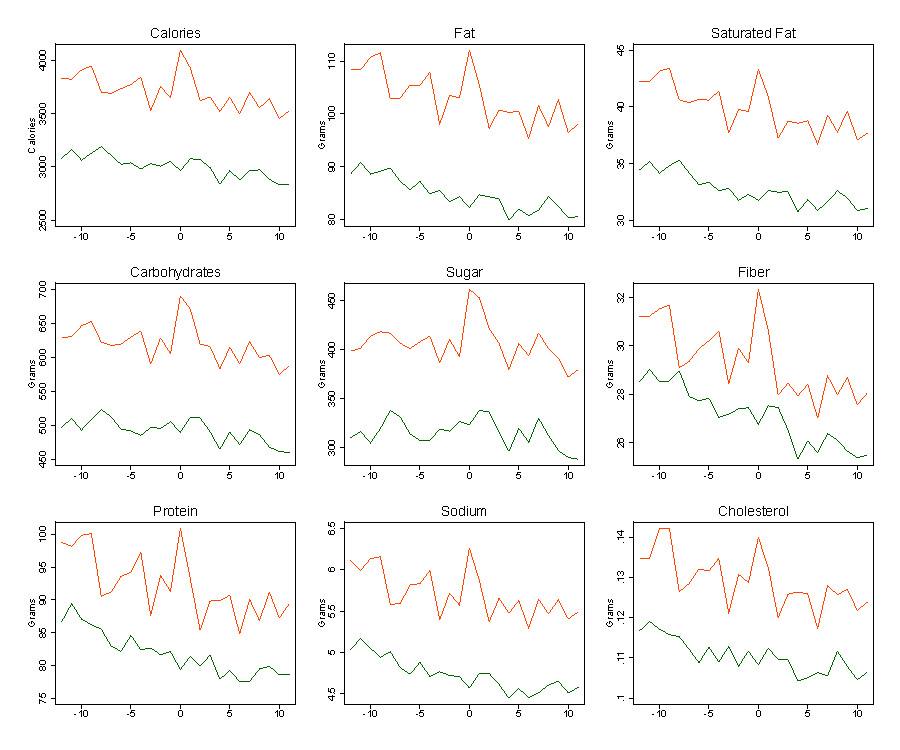
\includegraphics[width=1\textwidth, angle=0]{../figures/raw_nutrients_week.pdf}
\footnotesize Each panel displays weekly sums of different nutrients averaged across panelists in the sample by whether they have at least two months of income in liquid assets.
Orange (top) line is liquidity-constrained households, green (bottom) line is those with liquidity.
Averages are weighted by panelist projection factors provided by Nielsen.
\end{center}
\end{figure}

\end{document}
